%%%%%%%%%%%%%%%%%%%%%%%%%%%%%%%%%%%%%%%%%%%%%%%%%%%%%%%%%%%%%%%%%%%%%%%%%%%%%%%%%%%%
% Do not alter this block (unless you're familiar with LaTeX
\documentclass{article}
\usepackage[left=2cm,right=2cm,top=2.54cm,bottom=2cm,a4paper]{geometry}
\usepackage[onehalfspacing]{setspace}
\usepackage{amsmath,amsthm,amssymb,amsfonts, fancyhdr, color, comment, graphicx, environ}
\usepackage{xcolor}
\usepackage{mdframed}
\usepackage[shortlabels]{enumitem}
\usepackage{indentfirst}
\usepackage{hyperref}
\usepackage{listings}

\lstset{language=R,
    basicstyle=\small\ttfamily,
    stringstyle=\color{DarkGreen},
    otherkeywords={0,1,2,3,4,5,6,7,8,9},
    morekeywords={TRUE,FALSE},
    deletekeywords={data,frame,length,as,character},
    keywordstyle=\color{blue},
    commentstyle=\color{DarkGreen},
}


\hypersetup{
    colorlinks=true,
    linkcolor=blue,
    filecolor=magenta,      
    urlcolor=blue,
}

\pagestyle{fancy}

\newtheorem{theorem}{Theorem}
\newtheorem{lemma}{Lemma}
\newtheorem{assumption}{Assumption}
\newtheorem{proposition}{Proposition}
\newtheorem{definition}{Definition}

\theoremstyle{definition}
\newtheorem{thm}{Theorem}[section]
\newtheorem{lem}[thm]{Lemma}
\newtheorem{prop}[thm]{Proposition}
\newtheorem{cor}[thm]{Corollary}

\theoremstyle{definition}
\newtheorem*{defn}{Definition}
\newtheorem*{exmp}{Example}

\theoremstyle{remark}
\newtheorem*{rem}{Remark}
\newtheorem*{rec}{Recall}
\newtheorem*{note}{Note}
\newtheorem*{exer}{Exercise}
\newtheorem*{fact}{Fact}



%overset
\newcommand{\ovs}[2]{\overset{#1}{#2}}


\newcommand{\mat}[1]{\vec{#1}}
\newcommand{\set}[1]{\mathcal{#1}}
% transpose
\newcommand{\T}{\mathsf{T}} 
% inner product 
\newcommand{\ip}[2]{\left< #1,\, #2 \right>} 
% absolute value 
\newcommand{\abs}[1]{\left\lvert #1 \right\rvert} 
% norm 
\newcommand{\norm}[1]{\left\lVert #1 \right\rVert} 
% bar over text (to replace \bar and \overline)
\newcommand{\paren}[1]{\left( #1 \right)}

\newcommand{\mybar}[1]{\mkern 1.5mu \overline{\mkern -1.5mu #1 \mkern -1.5mu} \mkern 1.5mu} 
% hat over text (to replace \hat and \widehat)
\newcommand{\myhat}[1]{\mkern 1.5mu \widehat{\mkern -1.5mu #1 \mkern -1.5mu} \mkern 1.5mu} 
% tilde over text (to replace $\tilde and \widetilde)
\newcommand{\mytilde}[1]{\mkern 1.5mu \widetilde{\mkern -1.5mu #1 \mkern -1.5mu} \mkern 1.5mu}


% the set of all natural numbers 
\newcommand{\N}{\mathbb{N}} 
% the set of all real numbers 
\newcommand{\R}{\mathbb{R}} 
% the set of all real n-dimmensional vectors
\newcommand{\Rn}{\mathbb{R}^{n}} 
% the set of all complex numbers 
\newcommand{\C}{\mathbb{C}} 
% the set of all complex n-dimmensional vectors
\newcommand{\Cn}{\mathbb{C}^{n}}



\newenvironment{problem}[2][Problem]
    { \begin{mdframed}[backgroundcolor=gray!20] \textbf{#1 #2} \\}
    {  \end{mdframed}}

% Define solution environment
\newenvironment{solution}{\textbf{Solution}}

%%%%%%%%%%%%%%%%%%%%%%%%%%%%%%%%%%%%%%%%%%%%%
%Fill in the appropriate information below
\lhead{2021-28605}
\rhead{Dohyup Shin} 
\chead{\textbf{Advanced Statistical Method HW 4}}
%%%%%%%%%%%%%%%%%%%%%%%%%%%%%%%%%%%%%%%%%%%%%


\begin{document}

    \begin{problem}{6.1}
	Suppose that instead of the Poisson  model (6.1), we assume a binomial model 
    $$Pr\{x_k = x\} = \binom{n}{x}\theta_k^x(1-\theta_k)^{n-x},$$
    n some fixed and known integer such as n = 10. What is the equivalent of Robbins' formula (6.5)?

    \end{problem}
    
    \noindent
    \begin{solution}
    By Robbins' formula,  $\mathbb{E} ( \theta | x ) = \cfrac{\int_{0}^{1}\theta p_{\theta}(x) g(\theta) d\theta} {f_g(x)}$ where $f_g(x) = \int_{0}^{1}p_{\theta}(x)g(\theta)d\theta$. Then, 
    \begin{align*}
        \int_{0}^{1}\theta p_{\theta}(x) g(\theta) d\theta & = \int_{0}^{1} \binom{10}{x}\theta^{x+1}(1-\theta)^{10-x} g(\theta) d\theta\\
        & = \binom{10}{x} \paren{\int_{0}^{1} ( \theta^{x+1}(1-\theta)^{9-x} - \theta^{x+2}(1-\theta)^{9-x} )g(\theta) d\theta}\\
        & = \binom{10}{x} \paren{  f_g(x+1)/\binom{10}{x+1} -  \int_{0}^{1} \theta^{x+2}(1-\theta)^{9-x} g(\theta) d\theta  } \\
        & = \frac{x+1}{10-x} f_g(x+1) - \binom{10}{x} \paren{\int_{0}^{1} ( \theta^{x+2}(1-\theta)^{8-x} - \theta^{x+3}(1-\theta)^{8-x} )g(\theta) d\theta} \\
        & = \frac{x+1}{10-x} f_g(x+1) - \frac{(x+2)(x+1)}{(10-x)(9-x)}f_g(x+2) + \binom{10}{x} \int_{0}^{1} \theta^{x+3}(1-\theta)^{8-x} g(\theta) d\theta \\
        & = \cdots  \text{ (Continue this process)} \\
        & = \sum_{k = 1}^{10 - x} \cfrac{(x+k)(x+k-1)\cdots(x+1)}{(10-x)(9-x)\cdots(11-x-k)}(-1)^{k-1}f_g(x+k)\\
        & = \sum_{k = 1}^{10 - x} \cfrac{(x+k)!(10-x-k)!}{(10-x)!x!}(-1)^{k-1}f_g(x+k)
    \end{align*}
    Therefore,  the Robbins' formula is equivalent to $$\mathbb{E} ( \theta | x ) = \cfrac{1}{f_g(x)} \sum_{k = 1}^{10 - x} \cfrac{(x+k)!(10-x-k)!}{(10-x)!x!}(-1)^{k-1}f_g(x+k)  $$
    \end{solution}
    
  
    \begin{problem}{6.2}
    Define $\mathbb{V}\{ \theta|x \}$ as the variance of $\theta$ given $x$. In the Poisson situation (6.1), show that 
    $$\mathbb{V} \{ \theta|x \} = \mathbb{E} \{ \theta | x\} \cdot (\mathbb{E}\{\theta | x +1 \} - \mathbb{E}\{ \theta| x\}),$$
    where $\mathbb{E} \{ \theta | x\}$ is as given in (6.5).
    \end{problem}
    
    \noindent
    \begin{solution}
    By Robbins' formula, $\mathbb{E}( \theta|x ) = (x+1) \frac{f_g(x+1)}{f_g(x)}$, where $f_g(x) = \int_{0}^{\infty}p_{\theta}(x)g(\theta)d\theta$ is marginal distribution of x. Then, we know that $\mathbb{V}\{ \theta|x \} = \mathbb{E} ( \theta^2 | x ) - (\mathbb{E}(\theta| x))^2$. 
    So we'll show that $\mathbb{E} ( \theta^2 | x ) = \mathbb{E} (\theta | x) \cdot \mathbb{E}(\theta | x +1).$
    
    \begin{align*}
        \mathbb{E} ( \theta^2 | x ) & = \cfrac{\int_{0}^{\infty}\theta^2 p_{\theta}(x) g(\theta) d\theta} {f_g(x)} = \cfrac{\int_{0}^{\infty}\theta^2 \cfrac{\theta^x e^{-\theta}}{x!} g(\theta) d\theta} {f_g(x)} \\
        & =  (x+2)(x+1)\cfrac{\int_{0}^{\infty}\theta^{x+2} \cfrac{e^{-\theta}}{(x+2)!} g(\theta) d\theta} {f_g(x)} = (x+2)(x+1)\cfrac{f_g(x+2)} {f_g(x)}
        & = (x+2)(x+1)\frac{f_g(x+2)} {f_g(x)}\\
        & = (x+2)(x+1)\frac{f_g(x+2)} {f_g(x+1)} \frac{f_g(x+1)} {f_g(x)} 
          =  \mathbb{E}(\theta | x +1) \cdot \mathbb{E} (\theta | x)
    \end{align*}

    Therefore,  we have shown that the above equation holds.

    \end{solution}


    \newpage
    \begin{problem}{6.3}
    Instead of (6.8), assume $g(\theta) = (1/ \sigma) e^{-\theta/ \sigma} \text{ for } \theta > 0.$
    \begin{itemize}
        \item [(a)] Numerically find the maximum likelihood estimate $\hat{\sigma}$ for the Poisson model (6.1) fit to the count data in Table 6.1.
        \item [(b)] Calculate the estimates of $\hat{E} \{ \theta|x \}$, as in the third row of Table 6.1.
    \end{itemize}

    $$g(\theta) = \frac{\theta^{\nu -1}e^{\theta/\sigma}}{\sigma^{\nu} \Gamma(\nu)}, \text{for } \theta \geq 0
    , \quad (6.8)$$
    \end{problem}
    
    \noindent
    \begin{solution}
    \begin{itemize}
        \item [(a)] We'll find the maximum likelihood estimates of $\sigma$. Tha marginal probability density function of x is $f_g(x) = \int_{0}^{\infty} \cfrac{\theta^x e^{-\theta}}{x!}g(\theta)d\theta = \int_{0}^{\infty} \cfrac{\theta^x e^{-\theta}}{x!}(1/\sigma)e^{-\theta/\sigma}d\theta = \frac{\gamma^{x+1}}{\sigma} \int_{0}^{\infty} \cfrac{1}{\Gamma(x+1)\gamma^{x+1} }\theta^x e^{-\theta/ \gamma}d\theta \text{, where }\gamma = \frac{\sigma}{\sigma +1}$. Since the function in the integral follows Gamma(x+1, $\gamma$) distribution, $f_g(x) = \frac{\gamma^{x+1}}{\sigma} = \frac{\sigma^x}{(\sigma + 1)^{x+1}}$. So the marginal likelihood function of x is $L(\sigma) = \prod_{i = 1}^{N}f_g(x_i)$. Define the log likelihood function $l(\sigma) = log(L(\sigma)) = \sum_{i = 1}^{N} (x_ilog\sigma - (1+x_i)log(1+\sigma))$. The score function is $S(\sigma) = \dot l(\sigma) = -\frac{n}{\sigma + 1} + \frac{n \bar{x}}{\sigma} - \frac{n\bar{x}}{\sigma + 1}$ where $\bar{x} = \sum_{i = 1}^{N}x_i$. So we'll find the mle of $\sigma$ satisfying $S(\sigma) = 0$.
        $$S(\sigma) = 0 \Leftrightarrow -n\sigma + n\bar{x}(\sigma + 1) - n\bar{x}\sigma = 0 \Leftrightarrow -n\sigma + n\bar{x} = 0 \Leftrightarrow \sigma = \bar{x}$$
        Therefore, the mle of $\sigma$ is $\bar{x}$, denoted $\hat{\sigma} = \bar{x}$.
        So, we plug $\hat\sigma$ in $f_g(x)$. Then, 
        $$f_{\hat g}(x) = \cfrac{{\hat \sigma}^x}{{(\hat \sigma + 1)}^{x+1}}$$
        Actually, $\hat \sigma = \bar{x} = \frac{1}{9461}\sum_{i = 1}^{9461}x_i  = \frac{1}{9461}(1317\cdot1 + 239\cdot2 + 42 \cdot 3 + 14 \cdot 4 + 4 \cdot 5 + 4 \cdot 6 + 1 \cdot 7) = 0.2143537$
        Then,  $\hat y_x = 9461f_{\hat g}(x)$ where $x = 0, 1, \dots, 7$
        By using R, we can calculate $\forall y_x$.
        
        In summary, \\
        \begin{table}[h]
            \centering
            \begin{tabular}{|c|c|}
            \hline
            {\textbf{$\hat y_x$}} & {\textbf{Fitting value}} \\ \hline
            $\hat{y_0}$                         & 7790.976                        \\ \hline
            $\hat{y_1}$                         & 1375.237                        \\ \hline
            $\hat{y_2}$                         & 242.7523                        \\ \hline
            $\hat{y_3}$                         & 42.84982                        \\ \hline
            $\hat{y_4}$                         & 7.563708                        \\ \hline
            $\hat{y_5}$                         & 1.33512                         \\ \hline
            $\hat{y_6}$                         & 0.235671                        \\ \hline
            $\hat{y_7}$                         & 0.04159986                      \\ \hline
            \end{tabular}
        \end{table}
        

        \item [(b)] Since  $\hat{E} \{ \theta|x \} = (x+1) \cfrac{f_{\hat g} (x+1)}{f_{\hat g}(x)} = (x+1)\cfrac{\hat \sigma}{1 + \hat{\sigma}}$. So we can calculate the estimates of posterior mean for all $x = 0, 1, \dots, 6$
        
        \begin{table}[h]
            \centering
            \begin{tabular}{|c|c|}
            \hline
            \textit{\textbf{$\hat E(\theta | x) $}} & {\textbf{Fitting value}} \\ \hline
            $\hat E(\theta | x = 0) $               & 0.1765167                       \\ \hline
            $\hat E(\theta | x = 1) $               & 0.3530333                       \\ \hline
            $\hat E(\theta | x = 2) $               & 0.5295500                       \\ \hline
            $\hat E(\theta | x = 3) $               & 0.7060667                       \\ \hline
            $\hat E(\theta | x = 4) $               & 0.8825833                       \\ \hline
            $\hat E(\theta | x = 5) $               & 1.0591000                       \\ \hline
            $\hat E(\theta | x = 6) $               & 1.2356167                       \\ \hline
            $\hat E(\theta | x = 7) $               & $\cdot$                         \\ \hline
            \end{tabular}
        \end{table}

        The R code related to the above is attached to the last page.
    \end{itemize}
    
    \end{solution}

    \newpage
     
    \begin{problem}{6.7}
    The nodes data of Section 6.3 consists of 844 pairs $(n_i, x_i)$.
    \begin{itemize}
        \item [(a)] Plot $x_i$ versus $n_i$
        \item [(b)] Perform a cubic regression of $x_i$ versus $n_i$ and add it to the plot.
        \item [(c)] What would you expect the plot to look like if the values of $n_i$ were assigned randomly before surgery?
    \end{itemize}

    \end{problem}
    
    \noindent
    \begin{solution}

        (a)
        \begin{figure}[h]
            \begin{center}
            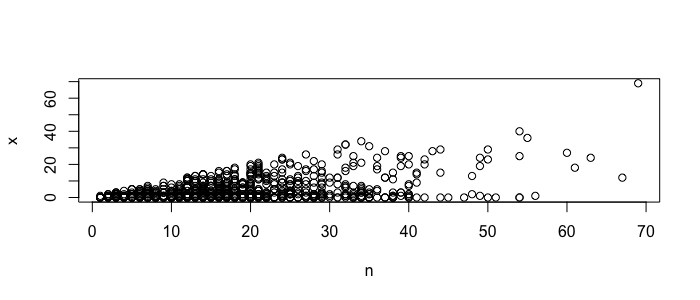
\includegraphics[width=4in]{./ASM_hw5_1.png}
            \end{center}
            \caption{}
        \end{figure}
        

        (b)
        \begin{figure}[h]
            \begin{center}
            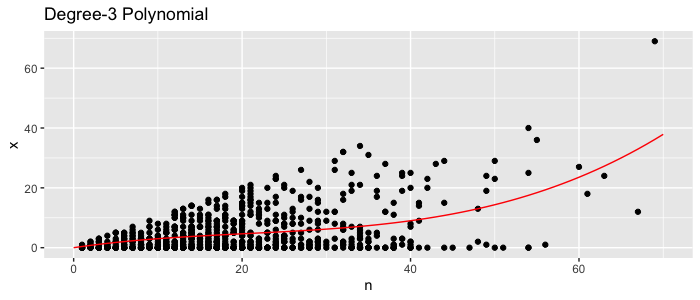
\includegraphics[width=4in]{./ASM_hw5_2.png}
            \end{center}
            \caption{}
        \end{figure}
        
    \end{solution}

    \begin{problem}{2}
        Show that the marginal distribution of "x"(in the missing species problem) is negative binomial.
    \end{problem}

    \begin{solution}
    In the book, the distribution of $x|\theta$ and $\theta$ are $x|\theta \sim Poisson(\theta)$ and $\theta \sim Gamma(\nu, \sigma)$. Then, the joint probability density function of $(x, \theta)$ is $f(x , \theta) = p_\theta(x)g(\theta)$ where $p_\theta(x)$ and $g(\theta)$ are pdf of $x|\theta$ and $\theta$.
    Then, the marginal pdf of x is 
    \begin{align*}
    f(x) & = \int_{0}^{\infty} f(x , \theta)d \theta = \int_{0}^{\infty} \cfrac{\theta^x e^{-\theta}}{x!} \cfrac{1}{\Gamma(\nu)\sigma^\nu}\theta^{\nu - 1}e^{-\theta/\sigma} d\theta \\
    & = \frac{\Gamma(x+\nu)\gamma^{x+\nu}}{\Gamma(\nu)x!\sigma^{\nu}}\int_{0}^{\infty}\cfrac{1}{\Gamma(x+\nu)\gamma^{x+\nu}}\theta^{x+\nu-1}e^{-\theta/\gamma} d\theta \quad (\text{where } \gamma = (1+\frac{1}{\sigma})^{-1}) \\
    & = \frac{(\nu+x-1)(\nu+x-2)\cdots(\nu + 1)\nu}{x!}(\frac{1}{\sigma + 1})^{\nu} (\frac{\sigma}{1+\sigma})^x \\
    & = \binom{x+\nu -1}{x}(\frac{1}{\sigma + 1})^{\nu} (\frac{\sigma}{1+\sigma})^x \quad \text{if $\nu$ is natural number}
    \end{align*}
    Therefore, if $\nu$ is natural number,  then the marginal pdf of x follows negative binomial distribution, denoted $Nebin(\nu, \frac{1}{1+ \sigma})$.
    
    \end{solution}


    \begin{problem}{3}
        Verify $E(t) = e_1\frac{1-(1 + \gamma t)^{-\nu}}{\gamma \nu}$ where $\gamma = (1/\sigma + 1)^{-1}$. (See the lecture note Chapter 6-2, page 5, parametric approach)    
    \end{problem}
    
    \begin{solution}
    In lecture note Chapter 6-2 page 5, we assume that the prior distribution of $\theta$ is $Gamma(\nu, \sigma)$.
    Let the pdf of $\theta$ be $g(\theta) = \frac{1}{\Gamma(\nu) \sigma^{\nu}} \theta^{\nu - 1} e^{-\frac{\theta}{\sigma}} $.
    The moment generating function of $\theta$ is $M_{\theta}(t) = E(e^{t\theta}) = (1-\sigma t)^{-\nu} \quad \forall t < \frac{1}{\sigma}$.
    To calculate $E(t)$, we use the mgf of $\theta$.
    
    \begin{align*}
     E(t) & = S\int_{0}^{\infty}e^{-\theta}(1 - e^{-\theta t}g(\theta)d\theta = S E(e^{-\theta}(1 - e^{-\theta t}))\\
     & = S(E(e^{-\theta}) - E(e^{-\theta (1+t)})) = S( (1+\sigma )^{-\nu} -(1 + \sigma(1+t))^{-\nu}  )\\
     & = S (1+\sigma)^{-\nu} (1 - (1 + \frac{\sigma}{1+\sigma }t)^{-\nu})\\
     & = S (1+\sigma)^{-\nu} (1 - (1 +\gamma t)^{-\nu})\\
    \end{align*}
    
    Next, we'll show that $e_1 = E(y_1) = S\gamma \nu(1+\sigma )^{-\nu}$. 
    \begin{align*}
         e_1 & = E(y_1)  = S\int_{0}^{\infty} \theta e^{-\theta}g(\theta)d\theta\\
         & =  S \cfrac{\Gamma(\nu + 1) \gamma^{\nu +1} }{\Gamma(\nu) \sigma^{\nu}} \int_{0}^{\infty} \cfrac{1}{\Gamma(\nu + 1)\gamma^{\nu + 1}}\theta^{\nu}e^{-\frac{\theta}{\gamma}} d\theta \\
         & =  S \cfrac{\nu \gamma^{\nu +1} }{\sigma^{\nu}} = S\nu \frac{{(\sigma/(1+\sigma))}^{\nu+1}}{\sigma^{\nu}} \\
         & = S\nu \frac{\sigma}{(1+\sigma)^{\nu + 1}} = S\nu \frac{\sigma}{1+\sigma} \frac{1}{(1+\sigma)^{\nu}} \\
         & = S\nu \gamma (1+\sigma)^{-\nu}
    \end{align*}
    
    Therefore, 
    $$E(t) = S(1+\sigma)^{-\nu}(1 - (1 + \gamma t)^{-\nu}) = e_1\frac{(1 - (1 + \gamma t)^{-\nu})} {\gamma \nu}$$
    \end{solution}
\end{document}

